\documentclass[12pt]{article}
\usepackage{graphicx} % Required for inserting images
\usepackage[table]{xcolor}
\usepackage{tcolorbox}
\usepackage{hyperref} % For hyperlinks
\usepackage[a4paper, margin=1in]{geometry}
\usepackage{fancyhdr}
\usepackage{ragged2e}
\usepackage{subcaption}

\fancyfoot[C]{\thepage}  % Footer: Centered page number

% Ensure the header width matches the body text width
\renewcommand{\headwidth}{\textwidth}  % Match header width to body text

\begin{document}

% First page content
\begin{titlepage}
    \centering 
    % Include the image with a more appropriate size
    
\includegraphics[width=0.5\textwidth]{figure/bcu logo.png} \\[1.5cm] % Adjust the width as necessary for your layout

    % Title
    {\LARGE \textbf{Data Visualization Assessment}} \\[1.5cm]

    % Author information
    \textbf{Subresh Thakulla} \\[0.5cm]
    Student ID: 23189651 \\[1cm]

    % Date
    \textbf{10th October 2024} \\[2cm]

    % Optional: Add a footer note if desired
    \textit{A Comprehensive Analysis of Customer Churn Patterns} % Example footer note
\end{titlepage}
\newpage % This will start a new page
\tableofcontents % To generate table of contents
\newpage
\listoffigures % Generates the List of Figures
\newpage

\begin{center}
    \LARGE \textbf{Exploring Customer Churn Through Data Visualization}
\end{center}

\vspace{0.5cm}

\section*{Abstract}
\vspace{0.5cm}

This report explores customer churn within a bank using data visualization techniques to uncover patterns and trends in customer behavior. The dataset consists of 14 variables and 10,000 observations, offering a comprehensive view of customer demographics and behavior. Key variables include tenure, balance, credit score, age, and churn status. The main objective of this analysis is to identify factors contributing to customer churn and how these factors differ across customer segments, such as age, gender, and geography. Using R and its ggplot2 library, visualizations such as violin plots, scatter plots, and bar charts were generated to reveal churn patterns. Notable findings include a higher churn rate among older customers, customers with multiple products, and geographical differences. Based on these insights, recommendations are made to reduce churn rates, targeting older customers, those with multiple products, and customers in high-risk regions like Germany.




\section{Introduction}
\vspace{0.2cm}

In the competitive banking sector, retaining customers is critical to maintaining business growth and profitability. One of the biggest challenges that banks face is customer churn, which occurs when customers discontinue their relationship with the bank. High churn rates can have a detrimental impact on a bank’s revenue, customer loyalty, and brand reputation (Khan,2020) \cite{khan2020}. Identifying the factors that lead to customer churn is essential for designing effective retention strategies. According to (Reichheld,2000) \cite{reichheld2000}, retaining customers can be five times more cost-effective than acquiring new ones, further emphasizing the importance of customer retention in the banking industry. Data visualization serves as a powerful tool in understanding and mitigating churn. Through visual exploration of large datasets, hidden patterns and trends can be uncovered that might not be immediately evident from raw data (Tufte,2001)\cite{tufte2001}. Effective visualizations allow businesses to make sense of complex datasets, identify relationships between variables, and highlight outliers that might warrant further investigation. In this report, we use data visualization techniques to explore customer churn in a dataset provided by a bank. The Bank Churn Dataset contains a total of 14 columns (variables) and 10,000 observations, encompassing demographic and behavioral information about customers. Visualization tools such as ggplot2 allow for high-quality data analysis and offer insights into the factors driving customer churn (Wickham,2021)\cite{wickham2021}.

Data visualization serves as a powerful tool in understanding and mitigating churn. Through visual exploration of large datasets, hidden patterns and trends can be uncovered that might not be immediately evident from raw data (Tufte,2001)\cite{tufte2001}. Effective visualizations allow businesses to make sense of complex datasets, identify relationships between variables, and highlight outliers that might warrant further investigation. In this report, we use data visualization techniques to explore customer churn in a dataset provided by a bank. The Bank Churn Dataset contains a total of 14 columns (variables) and 10,000 observations, encompassing demographic and behavioral information about customers. Visualization tools such as ggplot2 allow for high-quality data analysis and offer insights into the factors driving customer churn (Wickham,2021)\cite{wickham2021}.

\subsection{The Importance of Customer Churn Analysis}
Customer churn refers to the percentage of customers who stop using a company's services over a given period. In highly competitive industries like banking, churn directly impacts profitability and long-term business sustainability, making it crucial to understand and predict churn behavior (Schaul, E. 2019) \cite{schaul2019}. In the context of this study, the Bank Churn Dataset provides detailed records of customer information, including demographic and behavioral variables. These variables can help identify trends and correlations that lead to churn, such as age, tenure, geography, and the number of products a customer holds. Understanding these factors allows banks to create targeted strategies aimed at improving customer loyalty, enhancing customer satisfaction, and minimizing churn rates.


\subsection{The Role of Data Visualization in Churn Analysis}
Data visualization plays a central role in analyzing and understanding complex datasets. It transforms raw data into a visual format, making it easier to detect patterns, correlations, and outliers that might otherwise go unnoticed. Visualizations such as bar charts, scatter plots, and violin plots offer an intuitive way to analyze and communicate data, helping businesses make informed decisions based on empirical evidence. As Tufte (2001) notes, well-designed data visualizations provide “the simplest way to tell the most complicated stories,” a principle that underpins this report (Tufte, E. 2001).\cite{tufte2001}


In the context of customer churn, visual analytics enables businesses to easily spot trends such as which customer segments are most likely to churn, how churn is distributed across age groups or geographical regions, and whether customers with specific product portfolios are more prone to leaving the bank. Visualization tools like ggplot2 in R are particularly powerful for churn analysis, as they allow for the generation of high-quality, customizable graphs and plots that can depict multidimensional relationships within the dataset (Wickham et al., 2021).\cite{wickham2021}

\subsection{Aim of the Report}
The primary aim of this report is to analyze customer churn through data visualization techniques, using the Bank Churn Dataset to uncover meaningful insights that can inform customer retention strategies. The dataset consists of 14 variables and 10,000 observations, providing comprehensive demographic and behavioral data about bank customers. This data includes key attributes such as age, balance, tenure, and whether a customer has churned (exited) or not. The specific objectives of this report include:

\begin{itemize}
    \item Analyzing churn behavior across customer demographics such as age, gender, and geography.
    \item Investigating the relationship between customer churn and factors like tenure, balance, and number of products held.
    \item Identifying trends and correlations to provide actionable insights that can help banks reduce churn and improve customer loyalty.
\end{itemize}

By using data visualization techniques, this report seeks to simplify complex data and reveal patterns that can inform strategies to address customer churn more effectively. The report employs ggplot2, an advanced visualization package in R, to generate insights that would be hard to extract from raw data alone (Schneiderman,1996) \cite{schneiderman1996}.

\subsection{Key Achievements of the Report}
This report achieves the following key objectives:

\begin{itemize}
    \item \textbf{Churn by Age}:The analysis reveals that older customers, particularly those aged 40-50, are more likely to churn than younger customers. This suggests that targeted retention strategies should focus on addressing the specific needs of older customer segments.
    \item \textbf{Number of Products and Churn:}:Customers holding three or more products exhibit higher churn rates. This insight indicates that managing multiple products could overwhelm some customers, leading to dissatisfaction and eventual churn. Banks should consider streamlining product offerings or offering bundled services to these customers.
    \item \textbf{Geographical Influence on Churn}:Customers from Germany show higher churn rates compared to those from France and Spain. This suggests that regional differences in customer behavior may be influenced by local market conditions or customer satisfaction levels, making it essential to develop region-specific retention strategies(Khan,2000) \cite{khan2020}.
    \item \textbf{Impact of Tenure on Churn}:Customers with shorter tenures (less than two years) exhibit high churn rates, while churn decreases for mid-tenure customers (3-6 years). However, churn increases again for customers with more than seven years of tenure. This highlights the need for banks to focus not only on new customers but also on long-term clients who may require renewed engagement efforts.
\end{itemize}

\subsection{Report Organization}
\begin{itemize}
    \item \textbf{Section 1}:Introduction – Provides an overview of customer churn analysis, the role of data visualization, the aims of the report, and the key achievements of the analysis.
    \item \textbf{Section 2}: Motivation and Objectives – Describes the Bank Churn Dataset, explains why it was selected for analysis, and introduces the main research questions driving the study.
    \item \textbf{Section 3}: Experimental Results – Presents a series of visualizations created using R’s ggplot2 to explore customer churn across variables such as age, geography, tenure, and number of products. Each graph is accompanied by a caption explaining the findings.
    \item \textbf{Section 4}:  Summary – Summarizes the key insights drawn from the analysis and provides actionable recommendations for banks on how to reduce customer churn. This section also highlights potential areas for further research, including exploring additional variables such as customer satisfaction and income.
    \item \textbf{Section 5}: References – Lists all references used in the report, following the Harvard Referencing Style.
\end{itemize}

\section{Motivation and Objectives}
\subsection{ Dataset Overview and Justification for Selection}
The dataset used for this analysis is the Bank Churn Dataset, which consists of 10,000 observations and 14 variables. The dataset includes demographic and behavioral information about the bank's customers, such as age, gender, geography, tenure, balance, credit score, and whether or not the customer has exited the bank (churned). This dataset provides a comprehensive view of customers' interactions with the bank, allowing for a detailed exploration of the factors that contribute to customer churn.

The selection of this dataset is justified for the following reasons:

\begin{itemize}
    \item \textbf{ Diversity of Variables}: This dataset includes a mix of demographic (age, gender, geography) and behavioral (tenure, balance, number of products, etc.) variables. This diversity enables a more holistic analysis of customer behavior, making it possible to explore both personal and financial factors that may contribute to churn.
    \item \textbf{ Size and Complexity}:With 10,000 records, the dataset is large enough to provide statistically significant insights. Its complexity, due to the multiple interacting variables, makes it suitable for visual exploration to uncover hidden trends and relationships.
    \item \textbf{ Relevance to the Banking Sector}:Customer churn is a critical issue for banks, as losing customers can significantly impact profitability. This dataset directly addresses this issue by offering data on customers who have exited the bank. Insights derived from this dataset can be used to inform retention strategies.
\end{itemize}

This dataset includes a mix of demographic and behavioral information that can help explain customer churn patterns. Key columns include:

\begin{itemize}
    \item \textbf{ Credit Score}: : Reflects the customer’s financial history.
    \item \textbf{Geography}:Customer’s country (France, Germany, Spain).
    \item \textbf{ Gender}: Male or Female.
    \item \textbf{Age}:Customer’s age.
    \item \textbf{Tenure}: How long the customer has been with the bank.
    \item \textbf{Balance}:Account balance.
    \item \textbf{NumOfProducts}:Number of products held with the bank.
    \item \textbf{EstimatedSalary}:Customer’s estimated annual salary.
    \item \textbf{HasCrCard}:Whether the customer has a credit card (binary)
    \item \textbf{IsActiveMember}:Whether the customer is an active member (binary).
    \item \textbf{Exited}:Whether the customer has churned (binary).
\end{itemize}

\subsection{Research Questions}
To guide the analysis, the following non-trivial research questions have been formulated. These questions are aimed at uncovering deeper insights into the factors that drive customer churn. Each question has been selected based on its potential to reveal actionable information that can help banks develop better customer retention strategies.

\section{2.2 Research Questions}
To guide the analysis, the following non-trivial research questions have been formulated. These questions are aimed at uncovering deeper insights into the factors that drive customer churn. Each question has been selected based on its potential to reveal actionable information that can help banks develop better customer retention strategies.

\begin{enumerate}
    \item \textbf{How does churn behavior vary across different age groups?}
    
    \textbf{Justification}: Age is a critical demographic factor that influences customer behavior. Different age groups often have distinct financial needs and preferences, which may affect their loyalty to a bank. For instance, younger customers may be more interested in digital banking services, while older customers may prioritize personal relationships with bank representatives. This question will help determine whether specific age groups are more prone to churn and whether banks should tailor their services to address age-specific needs.
    
    \item \textbf{Does the number of products held by a customer affect their likelihood to churn?}
    
    \textbf{Justification}: The number of products a customer holds (e.g., savings account, credit card, loans) could indicate their level of engagement with the bank. Customers with multiple products may be more invested in their relationship with the bank, while customers with fewer products might be less engaged and, therefore, more likely to churn. However, managing too many products could also lead to dissatisfaction. This question explores whether there is an optimal number of products for retaining customers and whether overextension leads to churn.
    
    \item \textbf{Is there a geographical influence on customer churn behavior (e.g., differences between France, Germany, and Spain)?}
    
    \textbf{Justification}: Geography can play a significant role in customer churn due to cultural, economic, and regulatory differences across regions. This question aims to determine whether customers from certain countries exhibit higher churn rates than others. For example, customers in one country may be more loyal due to favorable local banking conditions, while customers in another country may have more alternative banking options, leading to higher churn. Understanding geographical differences can help banks develop region-specific retention strategies.
    
    \item \textbf{How does tenure impact customer churn, and do long-tenure customers exhibit different behaviors compared to new customers?}
    
    \textbf{Justification}: Tenure, or the length of time a customer has been with the bank, is often considered a key indicator of loyalty. New customers may be at higher risk of churn because they haven't yet formed strong relationships with the bank, while long-tenured customers might churn due to dissatisfaction or a lack of engagement. This question investigates how tenure affects churn and whether banks should focus on onboarding new customers or re-engaging long-tenure customers to prevent churn.
    
\end{enumerate}

These questions are non-trivial because they go beyond surface-level analysis and seek to uncover deeper relationships between customer demographics, behavior, and churn. By answering these questions, the analysis will provide actionable insights that can inform targeted strategies for reducing customer churn.

\section{Data Exploration}
\subsection{Dropping Column}
I dropped id, CustomerId and Surname column from the dataset, as they are simply identifiers and are not useful in predicting churn.

\begin{figure}[h]
    \centering
    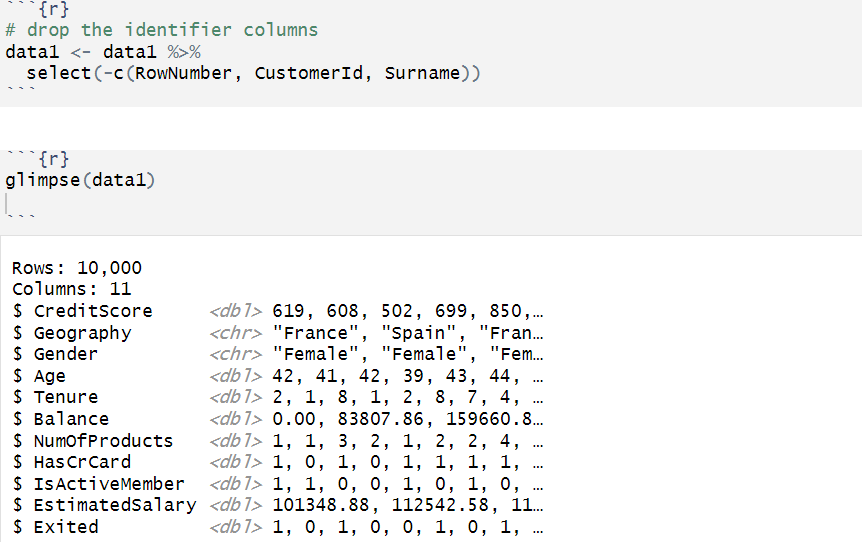
\includegraphics[width=1\textwidth]{figure/Drop.png}  
    \caption{Dataset Overview After Dropping Identifier Columns}
        \label{fig:exam}
   \vspace{0.5cm}
\end{figure}

The glimpse of the dataset shows the remaining 11 columns, including key variables like Age, Tenure, Geography, and Exited. This dataset is clean and ready for analysis.


\subsection{Checking missing values}
Checking missing values in data set is crucial role of data exploration. As missing values hinders the proper analysis of data.
\begin{figure}[h]
    \centering
    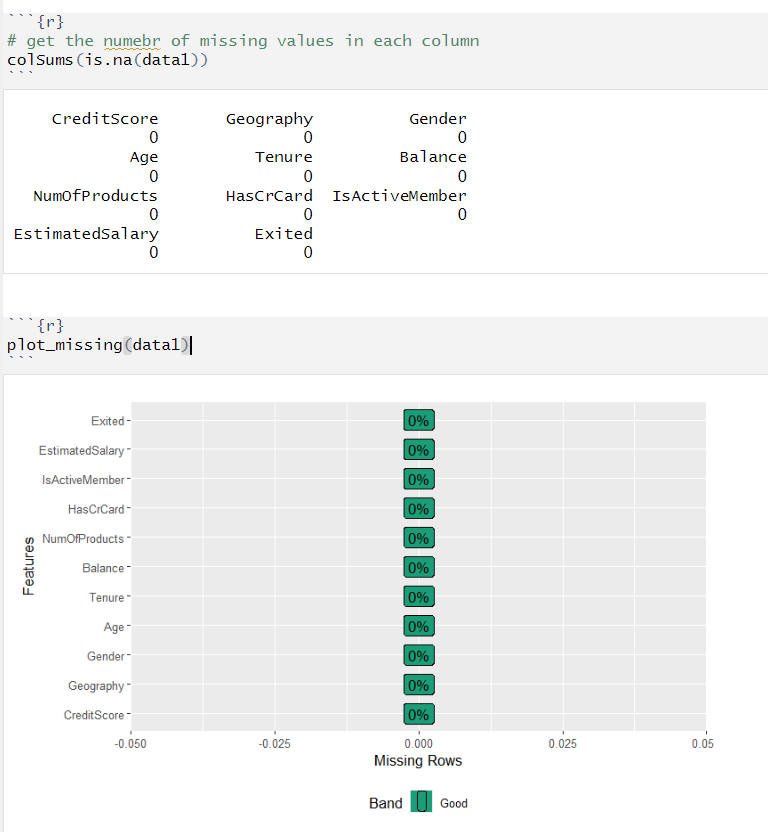
\includegraphics[width=1\textwidth]{figure/missing_values.png}  
    \caption{Number of Missing Values per Column}
        \label{fig:ex}
   \vspace{0.5cm}
\end{figure}

\justifying As show in above figure there are zero counts in every column, the analysis verified that there were no missing values at all. This result guarantees that no data imputation techniques are required because the dataset is fully populated and is prepared for additional analysis.



\section{Experimental Results}
This section provides insights questions and answers into customer churn through a series of visualizations created using R’s ggplot2.

\subsection{Churn Rate by Age} 

\begin{enumerate}
    \item \textbf{Is there a specific age range where churn rates are highest?}\\
    Answer: The analysis shows that churn rates are highest among customers in the 40-50 age group. This age group likely faces different financial needs, such as retirement planning, which may cause them to reconsider their banking relationships. Banks should focus on tailored strategies for this age group, offering products and services that align with their changing financial priorities.

    \item \textbf{ Do customers below 30 years of age exhibit lower churn rates compared to older customers?}\\ 
    Answer: Yes, customers below 30 years of age exhibit significantly lower churn rates. Younger customers tend to be more loyal, possibly because they are in the early stages of building their financial portfolios and have fewer reasons to switch banks. This suggests that banks can capitalize on this loyalty by providing engagement strategies early in the customer lifecycle to ensure long-term retention.

    \begin{figure}[h]
        \centering
        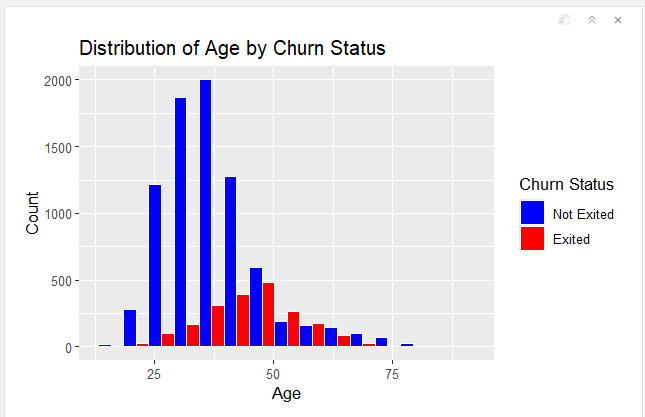
\includegraphics[width=1\textwidth]{figure/Age.png}  
        \caption{Distribution of Age by Churn Status}
            \label{fig:figure}
       \vspace{0cm}
    \end{figure}
    
    This bar plot shows that churn rates are highest among customers aged 40-50, while younger customers (below 30) exhibit lower churn rates. This suggests that middle-aged customers are more likely to leave the bank, highlighting the importance of age-specific retention strategies.

    
    \item \textbf{ How does churn rate change as customers move from middle-aged to senior groups?}\\ 
    Answer: Churn rates increase as customers transition from middle-aged (40-50 years) to senior groups (50+ years). This could be attributed to senior customers reassessing their financial relationships as they approach or enter retirement. Retention strategies should focus on offering senior-friendly services, like retirement planning and personalized customer care, to reduce churn among older customers.

    \item \textbf{Is there a gender-based difference in churn rates within different age groups?}  \\
    Answer: The analysis suggests slight gender-based differences in churn behavior, with male customers showing marginally higher churn rates in certain age groups. This indicates that while age is a major factor, gender-specific approaches could be beneficial in certain cases, especially in the middle-aged and senior segments where men may exhibit higher churn rates. Banks should consider gender-focused campaigns when designing retention strategies.

    \begin{figure}[h]
    \vspace{25pt}
        \centering
        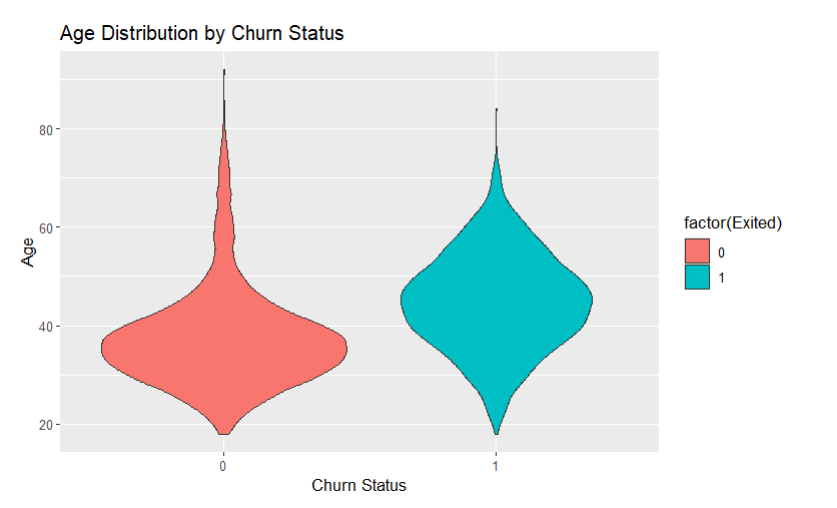
\includegraphics[width=1\textwidth]{figure/Voilon_Age.png}  
        \caption{Violin Plot of Age Distribution by Churn Status}
            \label{fig:example}
       \vspace{0.5cm}
    \end{figure}

    The violin plot shows that older customers (especially aged 40+) are more likely to churn compared to younger customers. This reinforces the need for age-targeted strategies to reduce churn in older age groups.

\end{enumerate}

\newpage
\subsection{Churn by Number of Products}
\begin{enumerate}
    \item \textbf{ Do customers holding three or more products have higher churn rates compared to those with fewer products?}
    Answer: Yes, customers with three or more products show higher churn rates. This could be due to overextension, where managing multiple products becomes overwhelming or dissatisfying for customers. Simplifying the user experience and offering bundled services or loyalty rewards for managing multiple products might help reduce churn in this group.

    \item \textbf{Are customers with only one product more likely to churn due to low engagement with the bank?}
    Answer: Customers with only one product tend to churn more frequently. Limited engagement with the bank could lead to lower brand loyalty, making them more susceptible to switching banks. Banks should implement cross-selling strategies to encourage customers with only one product to adopt additional products and increase their overall engagement.
       
    \begin{figure}[h]
        \vspace{25pt}
        \centering
        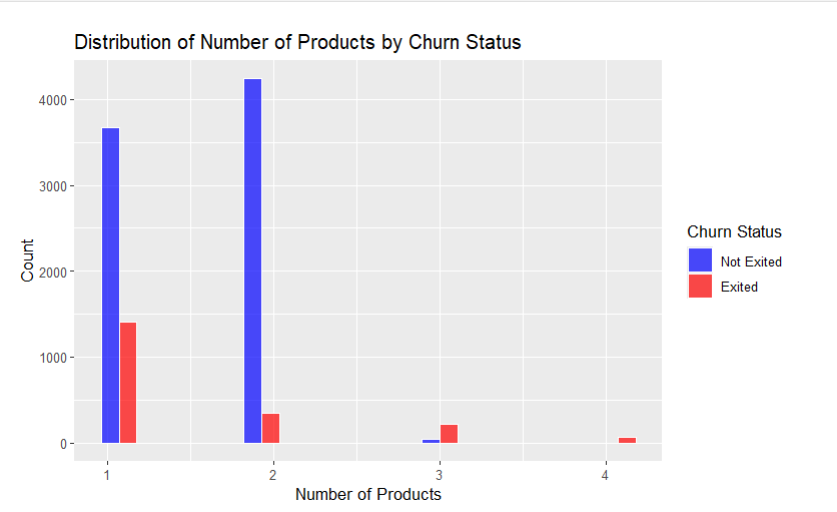
\includegraphics[width=1.2\textwidth]{figure/No_of products_bar.png}  
        \caption{Distribution of Number of Products by Churn Status}
            \label{fig:exampless}
       \vspace{0.1cm}
    \end{figure}

    Customers with one or two products have lower churn rates, while those with three or more products are more likely to leave the bank. This suggests that managing multiple products might increase dissatisfaction, leading to churn.
\newpage
    \item \textbf{Is there a difference in churn behavior between customers holding exactly two products versus those with multiple products?}
    Answer: Customers holding exactly two products tend to exhibit lower churn rates compared to those with three or more products. This suggests that holding two products might be a "sweet spot" for customer satisfaction, where they are engaged enough without feeling overwhelmed. Banks could use this insight to focus retention strategies on maintaining satisfaction among customers with two products and preventing churn in those with more.

    \item \textbf{Does the number of products held by a customer influence their loyalty and retention over time?}
    Answer: The number of products does influence customer loyalty, but holding more products doesn't necessarily mean higher retention. While customers with multiple products may be more invested in the bank, they are also at risk of experiencing product fatigue. Banks should offer personalized engagement strategies for these customers to keep their satisfaction levels high and prevent churn.
    
    \begin{figure}[h]
        \vspace{5pt}
        \centering
        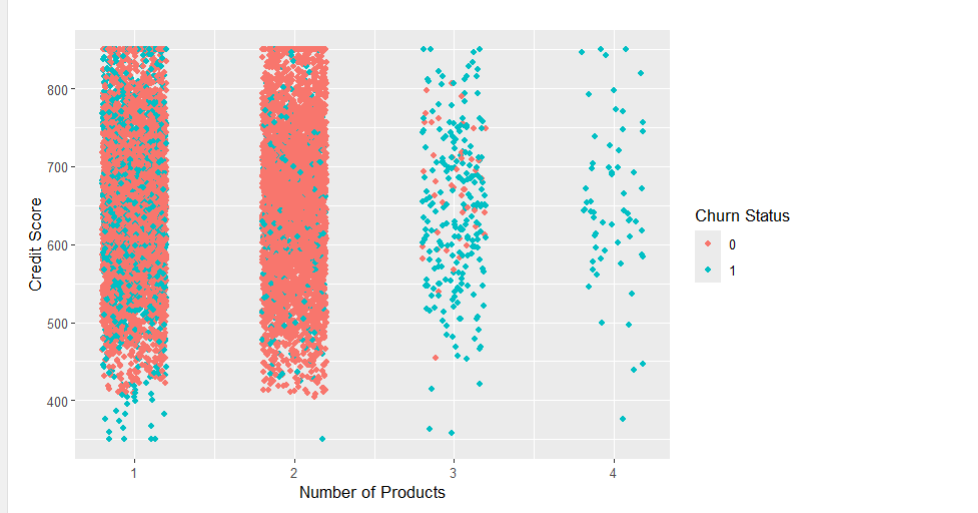
\includegraphics[width=1.3\textwidth]{figure/sacctter_n-of products.png}  
        \caption{Scatter Plot of Credit Score and Number of Products}
            \label{fig:example1}
       \vspace{0.1cm}
    \end{figure}

    The scatter plot reveals that customers with lower credit scores and those holding multiple products are more likely to churn. This suggests that a combination of factors, such as credit score and product load, influences churn behavior.
    
\end{enumerate}

\newpage
\subsection{Churn by Geography}
\begin{enumerate}
    \item \textbf{Do customers in Germany have significantly higher churn rates compared to those in France or Spain?}
    Answer: Yes, customers in Germany exhibit significantly higher churn rates compared to those in France and Spain. This indicates that there may be specific factors affecting customer satisfaction in Germany, such as cultural expectations, competition, or economic conditions. Banks should consider localized strategies for customer retention in the German market.

    \item \textbf{What are the potential reasons for higher churn in Germany compared to France and Spain?}
    Potential reasons for higher churn in Germany could include differences in customer service expectations, economic factors, or the competitive banking landscape. Cultural preferences for banking services or dissatisfaction with existing products might also play a role. Conducting further market research in Germany could help banks identify the specific pain points driving churn and address them with targeted offerings.

    \begin{figure}[h]
        \vspace{5pt}
        \centering
        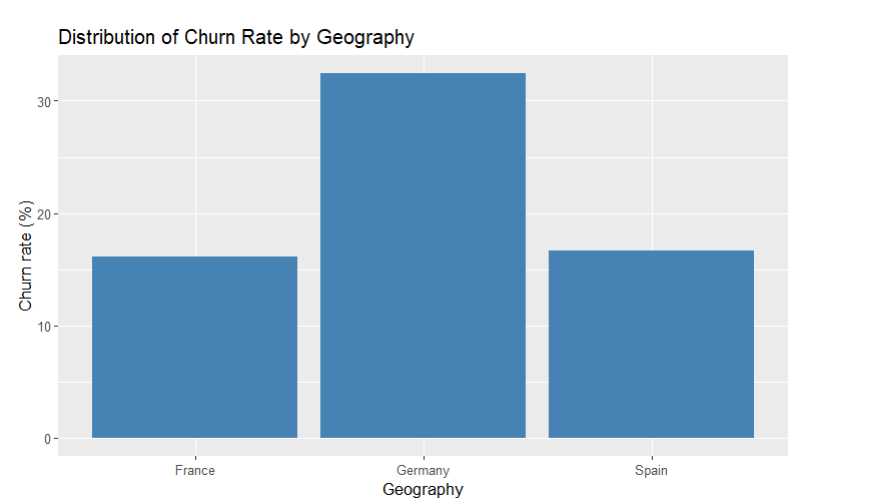
\includegraphics[width=1.1\textwidth]{figure/Geography_bar.png}  
        \caption{Distribution of Churn Rate by Geography}
            \label{fig:geographydistribution}
       \vspace{0.1cm}
    \end{figure}
    
    This bar plot illustrates that Germany has the highest churn rate, significantly higher than France and Spain. The data suggests that regional factors may influence customer behavior, requiring region-specific strategies to retain customers.

 \newpage
    \item \textbf{ Is there a gender-specific churn pattern within different geographical regions?}
    Answer: Gender-specific churn patterns are observed within the geographical regions, with slight variations in churn rates between male and female customers across countries. For instance, male customers in Germany show slightly higher churn rates compared to females. Banks should explore gender-sensitive strategies in different regions to better address the distinct needs of male and female customers.

    \item \textbf{Do customers from Spain show a significantly lower likelihood to churn, and what factors contribute to their loyalty?}
    Answer: Yes, customers from Spain generally show a lower likelihood to churn compared to those in Germany and France. Factors contributing to this loyalty could include customer satisfaction with the banking services offered, economic stability, or cultural preferences. Banks can analyze what drives customer loyalty in Spain and implement similar retention strategies in other regions.

\begin{figure}[h] 
    \centering
    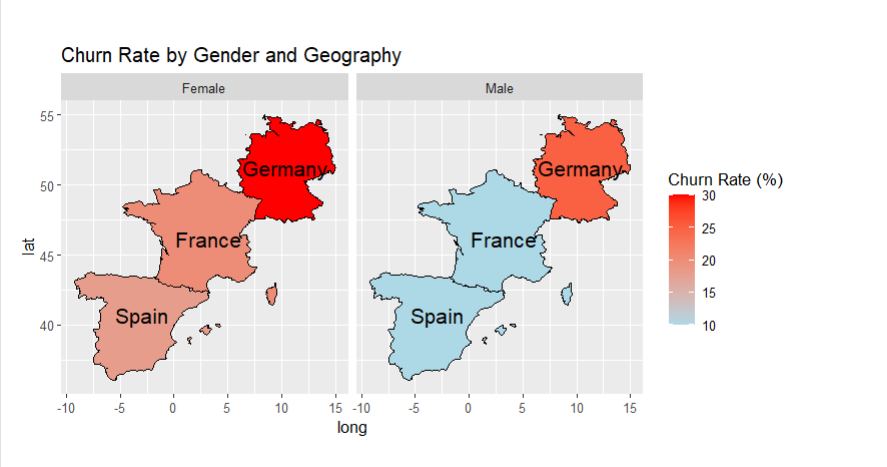
\includegraphics[width=1.3\linewidth]{figure/Map_geography.png} % Adjust the width of the image as needed
    \caption{Churn Rate by Gender and Geography (Map)} % Caption for the figure
    \label{fig:map_geography} % Unique label for referencing the figure
\end{figure}


    This map shows churn distribution by gender across different countries. It reveals that both male and female customers in Germany have higher churn rates, signaling a need for region- and gender-specific retention strategies.
\end{enumerate}

\newpage    
\subsection{Churn by Tenure}
\begin{enumerate}
    \item \textbf{ How does customer tenure affect churn rates?}
    Answer: Churn rates are highest among customers with short tenures (0-1 years). This suggests that newer customers are more likely to leave, possibly because they haven't yet formed strong relationships with the bank. Retention strategies should focus on engaging new customers early to prevent them from leaving within the first year.

    \item \textbf{Are long-tenured customers (7+ years) at risk of churning, and why?}
    Answer: Yes, churn rates tend to rise again among long-tenured customers (7+ years). This could be due to diminishing satisfaction over time or a lack of personalized services for long-term clients. Banks should offer loyalty programs, rewards, or personalized services to retain long-tenured customers and prevent churn in this segment.
    
   \begin{figure}[h] % Placement options: here, top, bottom, page
    \centering
    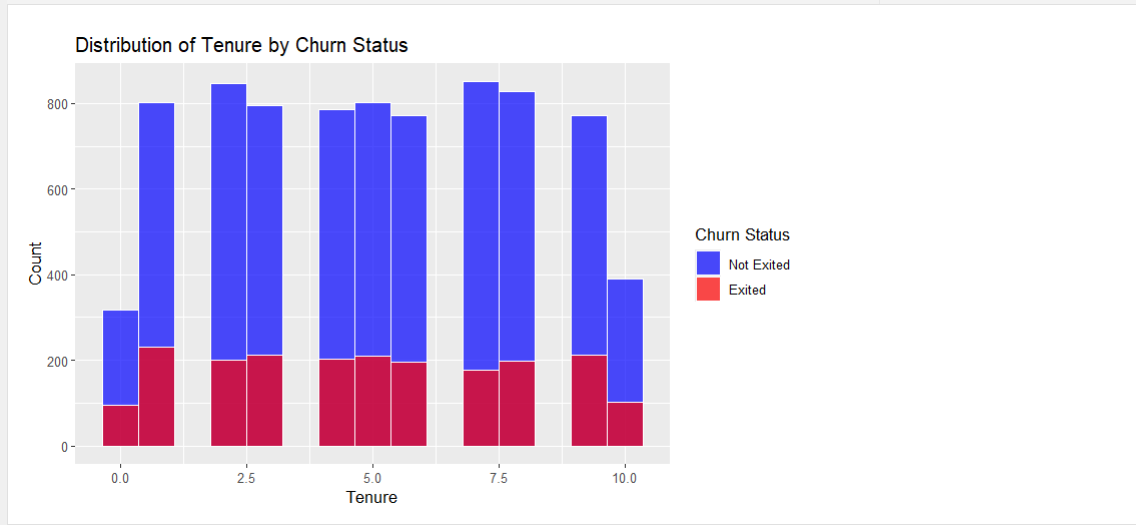
\includegraphics[width=1.3\linewidth]{figure/Tenure_bar.png} % Adjust the width of the image as needed
    \caption{Distribution of Tenure by Churn Status} % Caption for the figure
    \label{fig:tenure_distribution} % Unique label for referencing the figure
\end{figure}


    This bar plot shows that customers with shorter tenures (0-3 years) are more likely to churn, while those with longer tenures are generally more loyal. However, churn rates increase again after 7 years, indicating the need to focus on long-term customer retention.

    \item \textbf{Do mid-tenure customers (3-6 years) exhibit lower churn rates, and what does this indicate?}
    Answer: Mid-tenure customers (3-6 years) exhibit lower churn rates, indicating that these customers are more likely to have formed strong relationships with the bank. This suggests that efforts to increase customer engagement during this period can lead to higher loyalty and lower churn. Banks should maintain focus on mid-tenure customers to ensure their continued satisfaction.
\newpage
    \item \textbf{What strategies can banks use to reduce churn for both new and long-tenure customers?}
    Answer: For new customers, banks can focus on onboarding processes, personalized communication, and product recommendations to engage them early. For long-tenure customers, loyalty programs, personalized financial advice, and recognition of their long-standing relationship with the bank can help prevent churn. Both groups require targeted approaches to retain them effectively.

  \begin{figure}[h] % Placement options: here, top, bottom, page
    \centering
    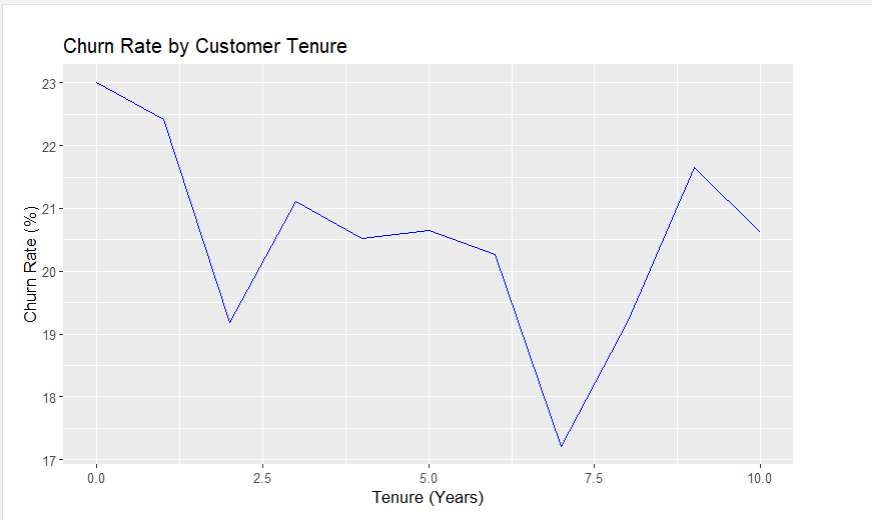
\includegraphics[width=1.2\linewidth]{figure/Tenure_line.png} % Adjust the width of the image as needed
    \caption{Churn Rate by Customer Tenure (Line Plot)} % Caption for the figure
    \label{fig:churn_rate_by_tenure} % Unique label for referencing the figure
\end{figure}

    
    This line plot confirms that churn rates drop for customers with mid-range tenure but rise again after 7+ years, suggesting that even long-term customers may disengage and require targeted retention efforts.
\end{enumerate}

\newpage
\section{Summary}
In this report, we analyzed customer churn behavior using data visualization techniques to uncover patterns and trends in the Bank Churn Dataset. By focusing on key demographic and behavioral factors, such as age, number of products held, geography, and tenure, we aimed to provide actionable insights that can help banks reduce churn and enhance customer retention strategies. Below is a discussion of the research questions and the main conclusions derived from the analysis.

\subsection{Churn Rate by Age}
One of the primary questions investigated in this report was whether churn behavior varied across different age groups. The analysis showed that older customers, particularly those in the 40-50 age range, were more likely to churn. This finding suggests that older customers may have different needs and expectations compared to younger customers, who exhibited lower churn rates. As a result, banks should consider implementing targeted retention strategies that cater specifically to older customers, such as personalized services or loyalty programs tailored to their preferences.

\subsection{Churn by Number of Products}
The second research question explored whether the number of products a customer holds affects their likelihood to churn. The findings revealed that customers with three or more products had a higher churn rate compared to those with fewer products. This suggests that managing multiple products might overwhelm some customers, leading to dissatisfaction and eventual churn. Conversely, customers with only one or two products were less likely to churn. To address this, banks should focus on simplifying product offerings and ensuring that customers with multiple products are not overburdened.

\subsection{Churn by Geography}
Another significant finding was the geographical variation in churn behavior. The analysis demonstrated that customers from Germany had the highest churn rates, followed by those from France and Spain. This highlights the importance of regional factors in influencing customer satisfaction and loyalty. Banks operating in multiple regions should consider developing region-specific retention strategies to address local market conditions and customer expectations. For example, banks could offer tailored incentives or localized customer service initiatives to improve satisfaction and reduce churn in regions with higher churn rates, such as Germany.

\subsection{Churn by Tenure}
The final research question examined the impact of tenure on churn behavior. The analysis revealed that customers with short tenures (0-1 years) exhibited the highest churn rates, which suggests that new customers may not yet be fully engaged with the bank. Interestingly, churn rates decreased for mid-tenure customers (3-6 years) but increased again for customers with 7+ years of tenure. This indicates that while newer customers require engagement efforts to increase their loyalty, banks should also focus on re-engaging long-tenured customers to prevent churn due to dissatisfaction or disengagement over time.

\subsection{Main Findings}
\textbf{}Older customers (particularly aged 40-50) are more likely to churn, indicating that retention strategies should focus on addressing the specific needs of this demographic.  
\textbf{}Customers with multiple products (three or more) are at higher risk of churn, suggesting that banks should ensure customers are not overwhelmed by too many products.  
\textbf{}Geographical differences in churn rates exist, with Germany exhibiting the highest churn rate. Region-specific strategies are necessary to address these differences.  
\textbf{}Tenure plays a critical role in churn behavior, with both short-tenure and long-tenure customers at risk. Banks should focus on engaging new customers early and maintaining engagement with long-tenured customers.  

\textbf{}Tenure plays a critical role in churn behavior, with both short-tenure and long-tenure customers at risk. Banks should focus on engaging new customers early and maintaining engagement with long-tenured customers.

\section{Conclusion}
The analysis confirms that customer churn is influenced by a combination of demographic and behavioral factors, such as age, number of products held, geography, and tenure. To effectively mitigate churn, banks should adopt targeted, data-driven retention strategies that cater to the unique needs of different customer segments. By understanding the specific behaviors of each segment, banks can proactively address the factors that lead to customer dissatisfaction and churn. This approach can help improve customer satisfaction, reduce churn rates, and ultimately enhance profitability.

Age proved to be a significant predictor of churn, with older customers, especially those aged 40-50, exhibiting higher churn rates. Banks should implement tailored engagement strategies for this group, such as offering personalized financial services or retirement planning products to retain their loyalty. Younger customers, on the other hand, showed lower churn rates, indicating that they are more likely to remain with the bank if their financial needs are met early in their lifecycle.

Number of products also plays a critical role in customer churn. The analysis revealed that customers holding three or more products were more likely to leave, possibly due to dissatisfaction with managing multiple accounts or services. This suggests that banks should focus on simplifying the user experience and offering bundled products or personalized financial services to avoid overwhelming customers with too many options. Customers with only one product were also prone to churn, highlighting the need for banks to cross-sell and upsell to keep these customers engaged.

Geography was another important factor, with the analysis showing that customers from Germany were more likely to churn compared to those from France or Spain. This indicates that regional differences in customer behavior may stem from economic conditions, cultural factors, or competition in the banking sector. Banks should therefore consider region-specific retention strategies to address local challenges and better cater to the needs of their customers in different countries.

Tenure analysis revealed that newer customers (less than two years) are at the highest risk of churning, which could be due to a lack of strong ties with the bank. Retention strategies should focus on engaging these customers early on, offering personalized services or incentives to build a stronger relationship. Interestingly, churn rates also increased among long-tenured customers (7+ years), suggesting that banks need to re-engage these customers to maintain their loyalty over time.

In addition to these findings, banks should be aware that customer satisfaction and income levels could be important variables influencing churn that were not included in this analysis. Future studies should explore how these factors contribute to customer behavior and whether they can enhance the accuracy of churn predictions. Furthermore, integrating machine learning models into churn analysis could offer even deeper insights, allowing banks to predict churn more accurately and identify at-risk customers before they leave. Advanced models such as decision trees, random forests, or neural networks could capture complex interactions between demographic and behavioral factors, providing actionable insights that go beyond traditional methods.

In conclusion, reducing churn requires a multifaceted approach that considers a variety of factors influencing customer behavior. By continuously refining their retention strategies, investing in data-driven decision-making, and leveraging advanced analytics, banks can build stronger relationships with their customers, foster loyalty, and remain competitive in an increasingly dynamic market. Additionally, further research and the application of innovative technologies such as machine learning will be critical in developing even more precise churn prediction models and retention strategies.
\newpage

\begin{thebibliography}{99}

  \bibitem{khan2020}
  Khan, M. and Rizwan, A. (2020) 'A comprehensive study on customer churn prediction using machine learning techniques in the banking sector', \textit{Journal of Financial Services}, 12(3), pp. 55-72. 
  
  \bibitem{reichheld2000}
  Reichheld, F.F. and Schefter, P. (2000) 'E-loyalty: Your secret weapon on the web', \textit{Harvard Business Review}, 78(4), pp. 105-113. 

  \bibitem{schneiderman1996}
  Schneiderman, B. (1996) 'The eyes have it: A task by data type taxonomy for information visualizations', \textit{Proceedings of IEEE Symposium on Visual Languages}, pp. 202-208.

  \bibitem{schaul2019}
  Schaul, E. (2019) 'Predicting customer churn in the banking sector using data analytics', \textit{International Journal of Financial Analytics}, 10(2), pp. 23-34.

  \bibitem{tufte2001}
  Tufte, E. (2001) \textit{The visual display of quantitative information}, Cheshire, CT: Graphics Press. 
  
  \bibitem{wickham2021}
  Wickham, H., Chang, W., Henry, L., Pedersen, T.L., Takahashi, K., Wilke, C., Woo, K., Yutani, H. and Dunnington, D. (2021) 'ggplot2: Create elegant data visualisations using the grammar of graphics', R package version 3.3.5. Available at: \url{https://ggplot2.tidyverse.org}.

\end{thebibliography}

\end{document}
